%%%%%%%%%%%%%%%%%%%%%%%%%%%%%%%%%%%%%%%%%%%%%%%%%%%%%%%%%%%%%%%%%%%%%%%%%%
% HEADER
%%%%%%%%%%%%%%%%%%%%%%%%%%%%%%%%%%%%%%%%%%%%%%%%%%%%%%%%%%%%%%%%%%%%%%%%%%

\pdfoutput=1

\documentclass[iop, apj, onecolumn]{emulateapj}

\usepackage{xspace}
\usepackage{amsmath}
\usepackage{framed} 
\usepackage{txfonts}
\usepackage{epstopdf}
\usepackage{graphicx}
\usepackage{color}
\usepackage{rotating}
\usepackage{natbib}
\usepackage{ulem}
\usepackage{xspace}
\usepackage[colorlinks=true,urlcolor=blue,linkcolor=blue,citecolor=blue]{hyperref}

\special{papersize=8.5in,11in}
\setlength{\pdfpageheight}{\paperheight}
\setlength{\pdfpagewidth}{\paperwidth}

%\input{commands}
%\input{macros}
%\input{citation_fix}

\shorttitle{Smoothing filter}
\shortauthors{More, S. \& others}

%\journalinfo{The Astrophysical Journal, {\rm 789:1 (18pp), 2014 July 1}}
%\submitted{Received 2014 January 6; accepted 2014 April 14; published 2014 June 9}
\slugcomment{Only submitted to the arXiv}

\begin{document}

%%%%%%%%%%%%%%%%%%%%%%%%%%%%%%%%%%%%%%%%%%%%%%%%%%%%%%%%%%%%%%%%%%%%%%%%%%
% EPS OR PDF FIGURES
%%%%%%%%%%%%%%%%%%%%%%%%%%%%%%%%%%%%%%%%%%%%%%%%%%%%%%%%%%%%%%%%%%%%%%%%%%

%%%%%%%%%%%%%%%%%%%%%%%%%%%%%%%%%%%%%%%%%%%%%%%%%%%%%%%%%%%%%%%%%%%%%%%%%%
% TITLE ETC
%%%%%%%%%%%%%%%%%%%%%%%%%%%%%%%%%%%%%%%%%%%%%%%%%%%%%%%%%%%%%%%%%%%%%%%%%%

\title{Extending the Savitzky Golay smoothing filter to data with covariant
errors}
\author{
Surhud More \altaffilmark{1}
}

\affil{
$^1$ Kavli Institute for the Physics and Mathematics of the Universe (WPI),
Tokyo Institutes for Advanced Study, The University of Tokyo,\\ 5-1-5 Kashiwanoha, Kashiwa-shi, Chiba, 277-8583, Japan;{\tt surhud.more@ipmu.jp}\\
}

%%%%%%%%%%%%%%%%%%%%%%%%%%%%%%%%%%%%%%%%%%%%%%%%%%%%%%%%%%%%%%%%%%%%%%%%%%
% ABSTRACT
%%%%%%%%%%%%%%%%%%%%%%%%%%%%%%%%%%%%%%%%%%%%%%%%%%%%%%%%%%%%%%%%%%%%%%%%%%

\begin{abstract}
Digital filters need to be commonly applied to noisy data for the purpose of
smoothing it and allowing a less noisy computation of the derivative. The
commonly used filter developed by Savitzky \& Golay based on a simplified least
squares procedure assumes equal errorbars on all data points. I present a simple
extension of this filter to heteroscedastic errors with covariance, a typical
case for many scientific datasets. A python implementation has been made
available at http://github.com/surhudm/savitzky\_golay\_with\_errors for ease of use.
\end{abstract}

\keywords{}

%%%%%%%%%%%%%%%%%%%%%%%%%%%%%%%%%%%%%%%%%%%%%%%%%%%%%%%%%%%%%%%%%%%%%%%%%%
% INTRODUCTION
%%%%%%%%%%%%%%%%%%%%%%%%%%%%%%%%%%%%%%%%%%%%%%%%%%%%%%%%%%%%%%%%%%%%%%%%%%

\section{Introduction}
\label{sec:intro}

The presence of noise in scientific data is unavoidable. The removal of noise
from data without degrading the underlying information is fundamental to
obtaining physical insights from the data. For cases, when detailed physical
models are absent or difficult to construct, it is useful to smooth the data, an
equivalent of the low pass filter in analog circuits.

\citet{SG1964} presented a simple numerical procedure for this purpose. Consider
data drawn from $y_i=f(x_i)+\epsilon$, where $\epsilon$ represents the noise,
and the index $i$ runs over the $N$ data points. The algorithm presented by
\citet{SG1964} considers a moving window (an odd integer, $2m+1$) centered
around the data point to be smoothed. The data is approximated as a polynomial
of degree $n$ around this point, whose parameters are determined using a least
squares procedure. The polynomial is then used to estimate the smoothed version
of the data. 
\begin{equation}
        y_{\rm SG}(x_i) = f^{\rm poly}_{n}(x_i|{y_i', i'\in[i-m,i+m]})
\end{equation}
The solution obtained by the minimization of least squares presented in
\citet{SG1964} does not use the estimates of the errors on the data (or
equivalently assumes equal errors on all data points without any covariance).
This results in a simple solution for the problem where the data has to be
convolved with a set of predetermined integers. This simple solution has been
implemented in many numerical libraries including python's numpy
(savgol\_filter) and has been used in the literature quite often (ADS suggests
1470 citations to the paper, Google scholar which perhaps tracks citations in
all the scientific fields suggests over 9000).

Although touted to be an optimal smoothing solution, the assumption of equal and
independent errors is quite rarely satisfied in real data. Therefore, I simply
recommend and extend this filter to use the errors whenever they are available.
I will show that in the case of data with heteroscedastic errors, using these
errors provides a much better description of the underlying signal than the
traditional Savitzky-Golay filter.

\section{Mathematical background behind the implementation}

The mathematical machinery behind the Savitzky Golay smoothing filter reduces to
the problem of fitting a $n^{\rm th}$ degree polynomial to a set of $(2m+1)$
data points with errors. This problem can be reduced to a matrix equation
involving the error weighted Vandermonde matrix of the abscissa of the data.
This is a well known problem in linear algebra, and various mathematical
libraries such as numpy in Python implement a solution to this problem. Many
of these libraries (for example, polyfit in  numpy.polynomial) however only
accepts errors without dealing with the covariance between these errors.

To overcome this issue, I reduce the problem of data with covariant errors to
one where the errors are independent. The $\chi^2$ metric for the polynomial
fitting problem with covariant errors is given by
\begin{equation}
        \chi^2 = \sum ({\bf y}-{\bf y}_{\rm model}[{\bf x}])^T {\bf C}^{-1}
        ({\bf y}-{\bf y}_{\rm model}[{\bf x}])\,,
\end{equation}
where
\begin{equation} 
        {\bf y}_{\rm model}({\bf x}) = {\bf a} {\bf V} {\bf x}\,.
\end{equation}
Here, ${\bf V}$ denotes the Vandermonde matrix, ${\bf a}$ denotes the $(n+1)$
coefficients of the $n^{\rm th}$ degree polynomial, and we seek those
coefficients which minimize the $\chi^2$.  The covariance matrix is a real
symmetric matrix and therefore allows an eigen decomposition, such that ${\bf
C}^{-1} = {\bf Q} \Lambda {\bf Q}^T$, where the columns of ${\bf Q}$ are
eigenvectors of ${\bf C}^{-1}$, and the diagonal elements of $\Lambda$ are its
eigenvalues. Therefore,
\begin{equation}
\chi^2 = \sum \left[{\bf Q}^T({\bf y}-{\bf y}_{\rm model}[{\bf x}])\right]^T
\Lambda {\bf Q}^T({\bf y}-{\bf y}_{\rm model}[{\bf x}])\,.
\end{equation}
The next step is to solve a modified problem: perform a polynomial fit to ${\bf
y'}={\bf Q}^T{\bf y}$ with errors given by the inverse of the square root of the
diagonal entries of $\Lambda$. The solution to this modified problem ${\bf a'}$
is then related to our desired solution ${\bf a}$ by ${\bf a}={\bf Q}{\bf a'}$.

We provide a convenient python routine which implements the above equations,
utilizes the standard polynomial fitting algorithm in the numpy library and
gives the optimally filtered data. This routine has been made available online.
\footnote{http://github.com/surhudm/savitzky\_golay\_with\_errors}

As a simple example let us consider data drawn from a sinusoid with
heteroscedastic errors. The traditional Savitzky Golay fit is compared to the
improved version in Figure~\ref{fig:improve}. It is clear that the traditional
smoothing filter is pulled away from the real solution by outliers which also
have larger errors associated with them. By accounting for these errors, the
improved filter presented in this work, provides a better alternative.

\begin{figure} 
        \centering{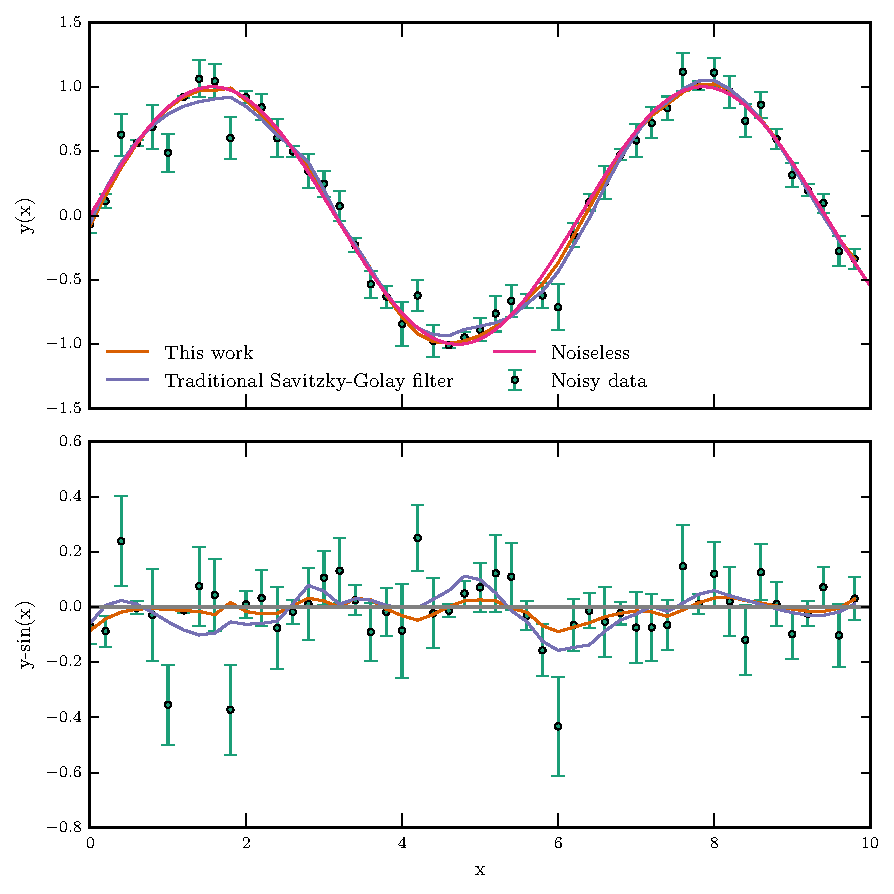
\includegraphics{Test_Sine.pdf}}
\caption{
        Data from a noisy $sin(x)$ curve filtered using the traditional
        Savitzky-Golay filter which assumes equal errors compared to the
        improved filter presented in this work which uses the actual errors on
        the data. Both the filters assume a window of 15 points and a fourth
        degree polynomial to fit the data. The improved filter performs
        significantly better and gives a much better representation of the data.
}
\label{fig:improve}
\end{figure}


%%%%%%%%%%%%%%%%%%%%%%%%%%%%%%%%%%%%%%%%%%%%%%%%%%%%%%%%%%%%%%%%%%%%%%%%%%
% BIBLIOGRAPHY
%%%%%%%%%%%%%%%%%%%%%%%%%%%%%%%%%%%%%%%%%%%%%%%%%%%%%%%%%%%%%%%%%%%%%%%%%%

\bibliographystyle{apj}
\bibliography{sf}
\end{document}
